\documentclass[onecolumn, 11pt, hmargin=1in, vmargin=1in]{aastex62}
%%%%%%begin preamble
\usepackage{hyperref}
\usepackage{url}
\usepackage{natbib}
\setlength{\bibsep}{0pt plus 0.3ex}
\usepackage{graphicx}
\usepackage{amsmath}
\usepackage{amssymb}

\usepackage{color}
\hypersetup{
  colorlinks   = true,
  %citecolor    = blue
  citecolor    = gray
  % gray is not being found!?!
  % gray is found if pdfpages is used... crap.
  %citecolor    = grey
  %citecolor    = Gray
}

%Copy+pasted from aastex.
\newcommand\prf{Phys.~Rev.~Fluids}     % Astrophysical Journal, Letters 
%% headers
\usepackage{fancyhdr}
\pagestyle{fancy}
\fancyhf{} % sets both header and footer to nothing
\lhead{Evan Anders---Research Statement}
\rhead{Stanford University, Stanford Science Fellows}
\cfoot{\footnotesize{\thepage}}
%\pagestyle{empty}
%\pagenumbering{gobble}
%\renewcommand*{\thefootnote}{\fnsymbol{footnote}}

\renewcommand{\vec}{\ensuremath{\boldsymbol}}
\newcommand{\dedalus}{\href{http://dedalus-project.org}{Dedalus}}
\newcommand{\del}{\ensuremath{\vec{\nabla}}}
\newcommand{\scrS}{\ensuremath{\mathcal{S}}}


%\usepackage{atbegshi}
%%%%%%end preamble


\begin{document}
\section*{}
\thispagestyle{fancy}

\begin{center}
\vspace{-1.45in}
\textbf{Motivation and Research Problem: The Solar Convective Conundrum}
\vspace{-11pt}
\end{center}

Stars are the cornerstone of studies in astrophysics and are themselves fascinating experiments where fluid dynamical processes occur at extreme parameters.
Asteroseismology measures sound and gravity waves at the surface of stars and, akin to seismic measurements on the Earth, traces the paths of those waves through the depths of the star to learn about its interior structure.
This technique enables the precise determination of age, mass, and radius of Sun-like stars, and these measurements are used across astrophysical disciplines like exoplanetary science and galactic archaeology \citep{huber&all2019}.
The interpretation of asteroseismic data relies on 1D models of stellar interiors which use decades-old parameterizations \citep{bohm-vitense1958} to deal with turbulent 3D processes like convection.
Stars like the Sun have convection zones near their surfaces, and these parameterizations and most modern simulations predict that ``giant cells'' characterized by large-scale horizontal motions are driven deep in those convective regions.
These giant cells are absent in observations of the Sun \citep{hanasoge&all2015}.
The absence of giant cells is called the ``Solar Convective Conundrum'' and implies that our most fundamental understanding of convection in stars is incomplete.
Sorting out this Convective Conundrum, and improving stellar models which are used broadly including in asteroseismic techniques, is crucial.



\begin{center}
\vspace{-5pt}
\textbf{Research Plan: Stellar Convection Across Spatial Scales}
\vspace{-11pt}
\end{center}
\begin{figure*}[b]
	\begin{center}
	\vspace{-8pt}
    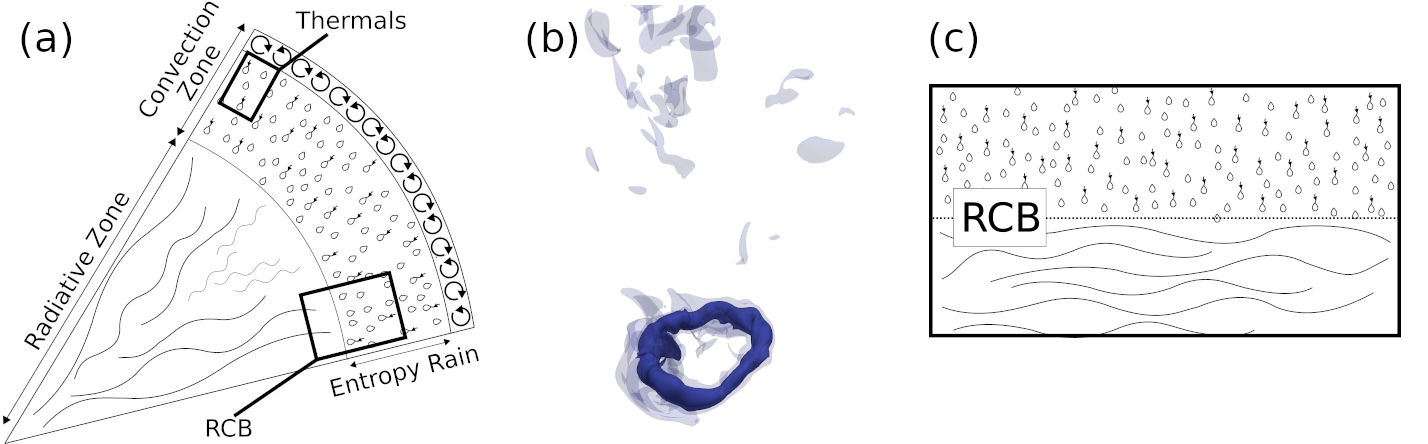
\includegraphics[width=0.95\textwidth]{./figs/tri_panel.png}
	\vspace{-8pt}
    \caption{ 
	(a) A schematic of the interior of Sun-like stars under the entropy rain hypothesis, where cold droplets of fluid carry the stellar luminosity below a small traditional convective surface layer.
	The scope of two experiments proposed here are boxed and labeled (``Thermals'' and ``RCB''), and the third experiment proposed here would contain the full spherical volume of the star, from which this wedge is taken.
	(b) A 3D visualization of entropy perturbations within the downward-propagating reference frame of a turbulent ``thermal,'' which models a stellar downflow.
	(c) A schematic of the radiative-convective boundary (RCB), where downflows impinge upon a stable layer and excite gravity waves within that layer.
	\label{fig:tri_panel} }
	\end{center}
\end{figure*}


Modern convective simulations reproduce flows at the Sun's surface reliably; deep convection, where giant cells would be driven, is still poorly constrained and understood.
During my time at Stanford, I will conduct a series of studies, outlined in Fig.~\ref{fig:tri_panel}, which span from the smallest to the largest scales in stellar convection.
I will progressively build on understanding gained in detailed small scale studies to inform studies which focus on increasingly larger scales.
As I have for my PhD, I will carry out my simulations using the Dedalus code \citep{burns&all2019}.

Stratified convection like that in the solar convection zone exhibits broad slow upwellings in balance with intense, fast downflows.
The now-popular ``entropy rain'' hypothesis posits that these downflows are so powerful that they alone transport the Sun's luminosity in the deep convection zone (see the schematic in Fig.~\ref{fig:tri_panel}a).
This hypothesis is gaining traction in recent simulations \cite{kapyla&all2017} and theoretical work \citep{brandenburg2016}, and could explain the absence of giant cells in observations \citep{hanasoge&all2015}.
These downflows may turbulently break up into distinct pieces as they fall and these individual downflow pieces can be modeled as ``thermals'' (a turbulent evolved thermal is visualized in Fig.~\ref{fig:tri_panel}b).
Thermals are studied extensively in Earth's atmosphere \citep{lecoanet&jeevanjee2019} and I recently studied them in the solar context \citep{andersLB2019}.

Regardless of the veracity of the entropy rain hypothesis, the nature of downflows in solar convection and their deep interactions must be better understood.
As a Stanford fellow, I will spend my first two years studying solar downflows to help clarify the convective conundrum.
In my first year, I will build on my work in \citet{andersLB2019} to understand how the Sun's magnetism and global rotation affect the propagation of individual downflows (thermals).
I will try to constrain whether or not Lorentz and Coriolis forces in the Sun can prevent downflows from transiting the full solar convection zone to help determine the importance of downflows and the plausibility of the entropy rain hypothesis.
Building on this work, my PhD studies of convection \citep{anders&brown2017, anders&all2019}, and sparse modern studies \citep{brummell&all2002, wood&brummell2018}, I will then examine interactions between downflows and the base of the solar convection zone, as in Fig.~\ref{fig:tri_panel}c.
The base of the convection zone in Sun-like stars is a radiative-convective boundary (RCB), where the turbulent convection zone meets a stably stratified ``radiative zone'' where radiation effectively carries the stellar luminosity.
In my second year, I will constrain the mechanisms through which an ensemble of downflows interacts with the RCB to understand how downflows pump energy, magnetic fields, and angular momentum into the radiative zone.
Giant cells should be driven near the RCB; mixing of near-RCB fluid by downflows may stablize the deep convection zone and prevent the acceleration of giant cell flows.
Furthermore, the topology of a star's angular momentum profile or magnetic field can affect asteroseismic measurements \citep{benomar&all2018, santos&all2018}, and so understanding how RCB interactions affect these topologies is crucial.

In my third year as a Stanford Science Fellow, I will zoom out from these detailed studies to examine full, spherical, global simulations of Suns; a partial wedge of such a sphere is depicted in Fig.~\ref{fig:tri_panel}a.
Recent studies \citep{jorgensen&weiss2019} have effectively coupled 3D simulations of thin, near-surface layers to 1D stellar structure models to improve measurements, but such a coupling is not yet available for deep convective motions.
Simulations of deep, turbulent convective motions take an unachievably large number of convective overturn timescales to come into an equilibrium state, and so cannot be efficiently coupled with 1D models while using traditional timestepping techniques due to computational expense.
In \citet{anders&all2018}, I developed a mechanism for coupling 3D simulations of deep motions and 1D boundary value problems (BVPs) to fast-forward these simulations to an equilibrated state.
During my time at Stanford, I will extend this work and design a generalized public module which couples 3D global simulations to 1D BVPs to reach a rapidly accelerated state.
I will personally employ this tool to create equilibrated global simulations; I will probe the nature of downflows and RCB interactions in these simulations and compare them to my previous more detailed studies to try to elucidate why modern observations and global simulations disagree so strongly about giant cells \citep{hanasoge&all2015}.
The implementation of this accelerated evolution tool will also be one of the next steps towards a generalized coupling of 1D stellar models and 3D convective simulations.
Such a generalized coupling, which samples 3D turbulent statistics of convection in order to inform and improve 1D modeling, is the ``holy grail'' of stellar structure modeling because it does not depend on simple parameterizations which have many known deficiences.


\begin{center}
\vspace{-5pt}
\textbf{How Stanford Enables These Accomplishments}
\vspace{-11pt}
\end{center}
Stanford is the perfect location for carrying out this work due to the opportunities available for interdisciplinary collaboration between astrophysicists, geophysical fluid dynamicists, applied mathematicians, and experts in turbulence.
The most natural collaborator on this work proposed here is Prof.~Tom Abel of Stanford's physics department.
Prof.~Abel's expertise in astrophysical fluid dynamics and scientific visualization, as well as his broad interest in astrophysical topics would make him an excellent collaborator for these proposed studies.
From Prof.~Abel's group, I would collaborate with the numerous experts in Stanford's Physics department, such as Prof.~Petrosian, who has recently studied the hydrodynamics of solar flares and Prof.~Wagoner, who has studied waves in astrophysical accretion disks.
There are many other natural collaborators with expertise in fluid dynamics across Stanford, such as Profs.~Sheshadri and Thomas in the Dept.~of Earth System Science and Profs.~Ryzhik and Tokieda in the Mathematics Department.
Finally, Stanford's Center for Turbulence Research, which houses many experts on turbulent fluid dynamics such as Prof.~Javier Jim\'{e}nez, will be an invaluable resource as I carry out my research plan.
This work will further be enabled by the computational resources available through Stanford's Research Computing Center, like the Sherlock HPC cluster.

The Stanford Science Fellows program would give me the freedom to study these ambitious problems in astrophysical fluid dynamics.
The projects proposed here seek to understand stellar convection from small to global scales and build naturally upon my PhD research.
These projects help solve exciting problems in stellar structure with applications in numerous astrophysical subdisciplines.
I look forward to the opportunity to create cross-disciplinary collaborations and carry on Stanford's excellent research tradition while making lasting contributions which help solve the Convective Conundrum and other fascinating problems. 

\vspace{-22pt}
\bibliographystyle{yahapj}
\bibliography{biblio}
\end{document}
